\section{模型检验：降维有效性与后段环境灵敏度}
\subsection{中截面、端部与整根积分}
\label{sec:dimension-validation}
中截面配对需要保持相同物性、环境与边界，才能识别额外轴向交换的影响。问题一80$\times$128二维对照在0--1800\unit{s}中截面采样的最大温度差约为$5.65\times10^{-8}\unit K$，含水率差约为$4.09\times10^{-9}\unit{kg/kg}$。问题二采用最终80$\times$256对照，在前10800\unit{s}的对应差为$1.69165\times10^{-3}\unit K$与$2.24706\times10^{-5}\unit{kg/kg}$，支持中截面工程近似，但不能宣称所有四位单元均一致。

另一方面，端面交换会改变整根失水。按二维控制体权重与一维圆环权重积分得到表\ref{tab:wholebody}。表中“失水增加”定义为$(C_0-\overline C_{2D})/(C_0-\overline C_{1D})-1$，不是平均含水率的相对误差。在空间均匀干密度的共同假设下，体积权重平均等于干质量权重平均。
\begin{table}[htbp]
\centering\small
\caption{同网格保存场的整根失水对照}\label{tab:wholebody}
\begin{tabular}{@{}lrrrr@{}}
\toprule 情形与时刻&二维网格&$\overline C_{2D}$&$\overline C_{1D}$&失水增加/\%\\\midrule
问题一，1800\unit{s}&80$\times$128&2.274929&2.293532&7.2533\\
问题二，3\unit{h}&80$\times$256&1.327482&1.382492&4.7118\\
问题四，6\unit{h}&80$\times$128&1.024545&1.065198&2.7379\\
\bottomrule
\end{tabular}
\end{table}

图\ref{fig:dimension-reduction}上排直接显示各时窗终点的中截面含水率差，下排并列对应的整根平均与失水增加，显示局部近似与总体失水应分别判断。上排各面板注明各自量级；下排各行时窗不同，只在同行的一维、二维之间作配对比较。
\begin{figure}[htbp]
\centering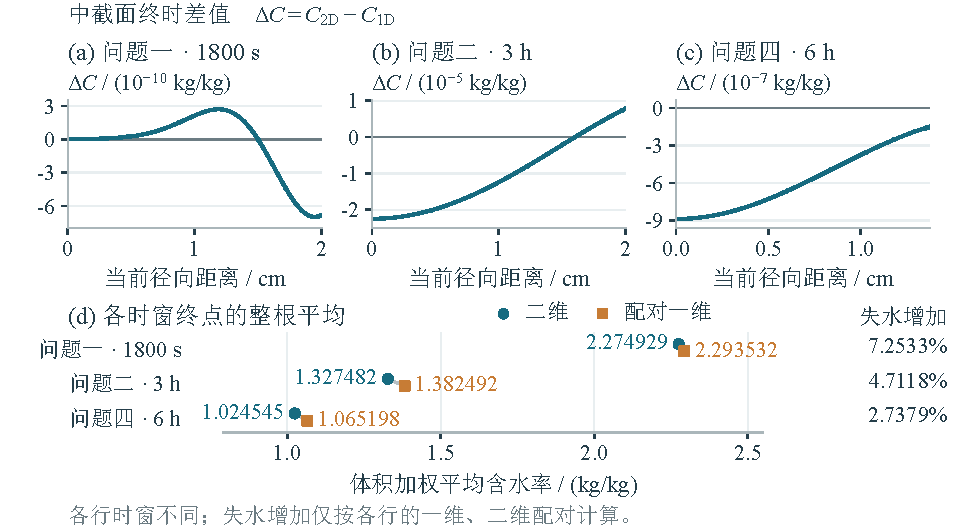
\includegraphics[width=.98\linewidth]{figures/legibility_validation/dimension_reduction.pdf}
\caption{已保存一维、二维配对场的降维证据：上排为问题一1800\unit{s}、问题二10800\unit{s}及问题四21600\unit{s}的中截面径向含水率差$\Delta C=C_{2D}-C_{1D}$；下排为各时窗终点的整根体积加权平均，圆点、方点分别表示二维和配对一维，终点失水增加与表\ref{tab:wholebody}一致。
问题一、二在已检时段中截面采样最大含水率差分别为$4.09\times10^{-9}$、$2.24706\times10^{-5}\unit{kg/kg}$。
上述时段最大差与上排终点差值的统计范围不同。
体积加权平均在空间均匀干密度假设下等于干质量加权平均。
数据取自同网格一维、二维配对保存场，文件索引与哈希见支撑材料图表来源清单；二维半柱坐标的$z=0$为中截面对称面。}
\label{fig:dimension-reduction}
\end{figure}
中截面差小与整根总量差可见并不矛盾。若用于全长平均、总失水或端部状态，应采用二维积分或明确忽略端面的近似，不能把中截面表格的精度扩展到全部工程指标。

上述中截面与整根积分对照用于评价降维近似，不能据此直接判定第四问的全域干燥终点。温度场与含水率相互耦合；即使$D$随温度增加，两个解之间的变系数通量散度也未必具有统一符号，因而不能将端面交换使干燥提前视为一般比较定理。

\subsection{后段环境的受控情景}
\label{sec:environment-scenarios}
由于式\eqref{eq:future}仅为4\unit{h}后的延拓，保持短时实测过程不变，从保存的4\unit{h}内部温湿场开展后段联立续算。每问设置原平台、温度$\pm1\unit K$和有效边界$b\pm0.005$五种情景；第四问始终使用同一观测$R(t)$。扰动幅度为人为选择的压力测试，没有作为测量不确定度或置信区间。表\ref{tab:environment}给出40阶配点的等号事件根，差值相对于同阶基线。
\begin{table}[htbp]
\centering\small
\caption{4\unit{h}后环境改变的条件根与时长差}\label{tab:environment}
\begin{tabular}{@{}lrrrr@{}}
\toprule 情景&问题三根/h&变化/h&问题四根/h&变化/h\\\midrule
原均值平台&57.473996&0&51.092003&0\\
$T_a-1\unit K$&59.341275&$+1.867279$&52.729346&$+1.637343$\\
$T_a+1\unit K$&55.688357&$-1.785639$&49.525343&$-1.566660$\\
$b-0.005$&57.382748&$-0.091249$&50.993818&$-0.098185$\\
$b+0.005$&57.584113&$+0.110117$&51.218753&$+0.126750$\\
\bottomrule
\end{tabular}
\end{table}
\begin{figure}[htbp]
\centering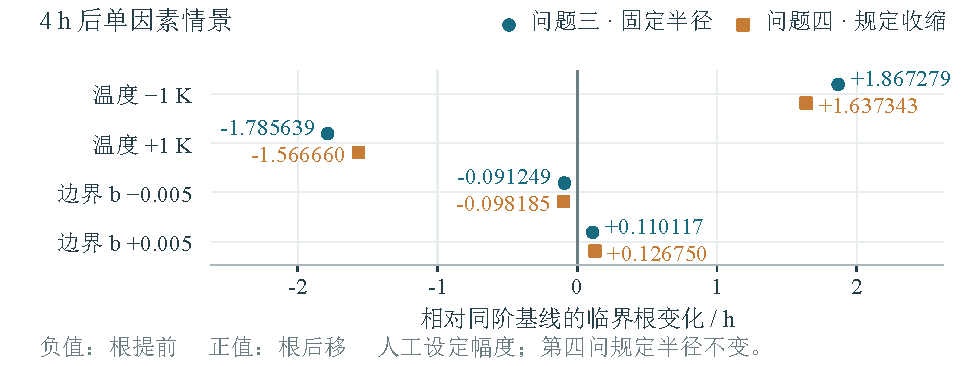
\includegraphics[width=.93\linewidth]{figures/legibility_validation/environment_sensitivity.pdf}
\caption{后段环境情景相对同阶基线的根变化；幅度为人工设定，第四问规定半径保持不变。圆点、方点分别表示问题三、四，共用零线；负值表示根提前，正值表示根后移。}\label{fig:environment}
\end{figure}
\FloatBarrier

对基线和降1\unit K情景进一步加密：问题三40阶到80阶、问题四40阶到60阶，单个根的最大变化分别约0.002951\unit{s}与0.000174\unit{s}，降温净效应的变化更小。因此小时级差不是此次降阶造成的；其他扰动没有逐一加密，表中六位小数仅便于追踪数值，不代表真实预测精度。

长期降温在既定模型内减小扩散温度因子，推迟阈值；提高$b$减小失水驱动力，也使根后移。由于两类扰动尺度不同，不能据图\ref{fig:environment}断定温度比所有湿度误差都重要。已有时间加权均值对照使问题三根变化约20.04\unit{s}，问题四改用PCHIP半径插值使根提前约12.61\unit{s}，二者也超过亚秒级一维经验数值预算。工程执行余量应建立在可用工况范围上，不能只依据四位小时的取整步长。

\section{模型评价、适用范围与推广}
\subsection{模型优点}
本文的优势体现在模型、数值实现与结果证据之间的对应关系，适用范围限于已声明的有效方程与工况。
\begin{enumerate}
\item \textbf{四问采用共同收支框架。}第\ref{sec:common-model}节统一热量、水分与材料运动的关系，各问再代入物性、几何和停止条件，便于区分变物性、终点判定与观测收缩的作用。
\item \textbf{圆环离散可核查总量收支。}第一问相邻控制体共享面通量，内部交换在求和时抵消，式\eqref{eq:q1-balance}将加权平均变化与表面交换对应，可用于检查离散总量一致性。
\item \textbf{原函数改写保持扩散通量。}式\eqref{eq:primitive}把可分离扩散率写为温度因子与原函数梯度的乘积，允许插值较平缓的原函数后反求含水率，保留题给非线性关系。
\item \textbf{终点判断兼顾内部极值与时间裕量。}式\eqref{eq:q3-extrema-candidates}--\eqref{eq:q3-reconstructed-max}检查径向重构的全部实驻点及端点，式\eqref{eq:event}区分等号临界根与严格执行时刻，避免用已舍入表值代替阈值判断。
\item \textbf{材料坐标避免重复计入收缩。}第\ref{sec:q4}节由组分守恒推导固定参考域方程，干基含水率无额外浓缩项；无交换纯收缩检验保持初态温湿与干、水质量，与所选材料运动一致。
\item \textbf{验证与输出来源分层可追溯。}第\ref{sec:q1}、\ref{sec:q2}节以独立算法和加密结果交叉核验，规定表值由对应未舍入数组生成；二维节点、配对估计与连续严格界分开报告，便于辨认结论由哪一级证据支持。
\end{enumerate}

\subsection{模型推广}
\label{sec:model-extension}
对具有同类有效物性与交换系数的圆柱形农产品，可将物性公式、环境记录和目标含水率作为替换接口，沿用控制体收支、离散组装与终点检测流程；迁移前须核对参数的单位、质量基准及适用温湿区间。本文未用其他物料作验证。

几何推广可从第\ref{sec:dimension-validation}节的一维径向与轴对称二维配对出发，在共同收支方程中替换散度算子、控制体权重及边界面。其他几何仍须重新处理对称条件、表面交换和网格检验，不能沿用本题的降维精度。对于以空间最大值限制工艺终点的其他状态量，若有可求极值的空间重构和明确的时间穿越方向，可移植“空间极值搜索、等号根定位、执行裕量复核”的事件流程，并按该变量重新设置阈值与误差预算。

对于已知外半径历程的物料，可用材料坐标组织输入，并按干物质守恒建立随动权重；内部运动仍需独立依据，仅有外半径不能唯一确定内部变形。取得后段工况记录后，第\ref{sec:environment-scenarios}节的单因素情景框架可用于比较允许工况范围内的终点变化，为工艺余量选择提供条件依据；本题人工扰动幅度不直接移作其他物料的余量。

\begingroup
\setlength{\parskip}{0pt}
\subsection{适用范围与主要限制}
\label{sec:limitations}
题表距离按中截面径向解释并作二维校核，并非题面指定的位置。

\textbf{气固边界与目标可达性。}材料$C$与空气$y_a$即使同写\unit{kg/kg}，分母也未必相同；湿度比、相对湿度与蒸气浓度须区分\cite{ashrae}。真实气膜候选边界为
\begin{equation}
j_s=k_g\{c_{v,s}(C_s,T_s)-c_{v,a}\},
\label{eq:physical-interface}
\end{equation}
其中$c_{v,s}$需材料水活度或解吸关系。仅当$c_{v,s}-c_{v,a}\approx K(C_s-b)$时，才能建立$\rhod h_m=k_gK$，不能直接交换系数数值。相关模型采用平衡干基含水率或气相/解吸关系\cite{dasilva2014,adrover2020}，未提供本药材标定值。须先核实目标环境下$C_{\mathrm{eq}}<0.15$；若$C_{\mathrm{eq}}\ge0.15$，从较高含水率开始的扩散干燥可能无法实现全域严格阈值，加密网格不能消除不可达性，未经标定的边界情景也不能称为实测。

\textbf{经验密度与材料质量的相容性。}若将题给$\rho=a+b_\rho C$同时解释为真实当前湿体密度，干基定义要求
\begin{equation}
\rhod(C)=\frac{a+b_\rho C}{1+C},\qquad
\frac{\dd\rhod}{\dd C}=\frac{b_\rho-a}{(1+C)^2}.
\end{equation}
这与前三问固定骨架的恒定干密度、第四问仿射收缩的空间均匀干密度不相容。本文仅将题给$\rho$用于有效容量，是建模处置而非题面规定。按第四问保存场强制采用真实湿密度解释，7\unit{h}和末态隐含干质量相对初值为0.71952、0.89029；保持$C,R$场不变，凑足总干质量需使长度由25\unit{cm}增至34.7454\unit{cm}与28.0807\unit{cm}。轴向收缩不能修复缺口，伸长凑平总量也未解决局部相容性；该反例不等于独立干质量账本数值泄漏，也不是可行伸长模型。

\textbf{相变能量与可报告的指标。}式\eqref{eq:heat}未显式计入相变能量，有限的$\rhoe c_p$不能在近等温持续失水时自动补充汽化功率。在“初始湿密度确定干质量、全部等效失水均蒸发”的附加条件下，取诊断常数$\lambda=2.45\unit{MJ/kg}$\cite{fao}，问题一1800\unit{s}的潜热需求约45.59\unit{kJ}，原轨迹对流输入约4.801\unit{kJ}，比例约9.50。问题四12\unit{h}表面近于环境温度、原轨迹净对流输入接近零，条件潜热通量$\lambda\rhod h_m(C_s-b)$仍约164.10\unit{W/m^2}。这些量级表明相变能量缺口尚未闭合，并非实际热量测量；重新联立相变会改变表面温度、热输入和扩散，不能固定原热输入倍乘干燥时间。现稿可报告有效模型的温湿分布、阈值事件和条件时长差，不能据此推断真实热量收支或执行保证。

\textbf{数值证据与工况的适用层级。}第三问57.4741\unit{h}的工程保守方向由二维终点节点场和配对根差支持，局部续算继承的前史误差仍需区分，不能将该时长解释为精确的二维最短时间；第四问51.0921\unit{h}为所设条件下的一维径向模型执行时长，已有粗网格二维核查在该时刻的最大含水率略高于阈值，有限圆柱全域达标尚待进一步验证，相关记录见支撑材料。两问均未取得连续二维严格误差界，也不能把条件时长作为实际工况保证。后段人为情景的幅度与用途见第\ref{sec:environment-scenarios}节，数值余量不覆盖环境、气固映射与物性假设的不确定性。
半径重建方案间的差异属于输入处理敏感性，不给出测量置信区间；复现规定的观测半径也不验证温湿预测，改变工况而沿用该历程时仅能报告条件响应。
\par\endgroup
